\documentclass[11pt]{article}
\usepackage[utf8]{inputenc}
\usepackage[T1]{fontenc}
\usepackage[final]{pdfpages} 
\usepackage[french]{babel}
\usepackage{amsmath}
\usepackage[bookmarks={true},bookmarksopen={true}]{hyperref}
\usepackage{graphicx}
\usepackage[a4paper]{geometry}
\usepackage{tikz}
\usetikzlibrary{shapes}
\usepackage{listings}
	\lstset{frame=tb,
		language=Java,
 		aboveskip=3mm,
  		belowskip=3mm,
  		showstringspaces=false,
  		columns=flexible,
  		basicstyle={\small\ttfamily},
  		numbers=none,
 		numberstyle=\tiny\color{gray},
  		keywordstyle=\color{blue},
  		commentstyle=\color{dkgreen},
  		stringstyle=\color{mauve},
  		breaklines=true,
  		breakatwhitespace=true
  		tabsize=3
	}
\pagestyle{plain}
\setlength{\parindent}{5mm}

\usepackage{color}

\definecolor{dkgreen}{rgb}{0,0.6,0}
\definecolor{gray}{rgb}{0.5,0.5,0.5}
\definecolor{mauve}{rgb}{0.58,0,0.82}



\title{\textbf{Projet LSINF1121 -  Algorithmique et structures de données\\ - \\ Rapport intermédiaire Mission 3} \\ {\large Groupe 3.2}}
\author{Boris \bsc{Dehem} \\(5586-12-00)\and Sundeep \bsc{Dhillon} \\(6401-11-00)\and Alexandre \bsc{Hauet} \\ (5336-08-00) \and Jonathan \bsc{Powell}\\(6133-12-00)\and Mathieu \bsc{Rosar} \\ (4718-12-00)\and Tanguy \bsc{Vaessen} \\ (0810-14-00)}
\date{date}
\date{\vspace*{25mm}

\includegraphics[scale=0.75]{logo.jpg}\\
		\vspace*{30mm}
		\begin{center}
		Année académique 2014-2015 \\	
		\end{center}}

\begin{document}
\thispagestyle{empty}

\maketitle
\thispagestyle{empty}
%\tableofcontents
%\setcounter{tocdepth}{3}
%\setcounter{page}{1}
%\newpage
\section*{Questions et réponses}

\subsection*{Question 1}
%%Énoncé
Énoncé

%%Réponse
Réponse
\newpage
\subsection*{Question 2}
Un arbre binaire de recherche présente-t-il un avantage par rapport à une table de hachage pour réaliser un \textit{Map} ? Pourquoi ? Et par rapport à une \textit{Skip List} ? \\
La forme d’un arbre binaire de recherche dépend-elle de l’ordre d’insertion des clés ? La forme d’un arbre binaire de recherche dépend-elle de l’ordre de suppression des clés ? Quelle est la complexité temporelle de l’insertion de $\textit{n}$ clés identiques dans un arbre binaire de recherche initialement vide ? Quelle est la propriété particulière des arbres binaires de recherche qui justifie l’intérêt d’autres structures de données comme les Arbres AVL ou les Arbres (2,4) ? (\textbf{Sundeep}) \\
\bigskip

Si on utilise un arbre binaire de recherche, l'avantage principal est lié à l'efficacité des méthodes qui ne seront plus en complexité temporelle $O(n$) mais bien en $O(log (n))$ dans le meilleur des cas et ce, surtout si l'arbre est équilibré. Au contraire, dans le pire des cas, la complexité temporelle sera en $O(n)$ vu que l'arbre n'est pas du tout équilibré et donc, la hauteur est de $n$. \\

Face à une \textit{Skip List}, cet avantage n'en est plus un vu que la complexité temporelle dans ces deux cas est identique. \\ 

La forme d'un arbre binaire de recherche dépend effectivement de l'ordre dans lequel on ajoutera ou supprimera des clés. Si l'on ajoute les clés dans l'ordre croissant (ou décroissant), l'arbre ne sera dans plus du tout équilibré et aura une hauteur de $n$. La meilleure chose à faire serait d'ajouter les différentes clés en prenant les clés centrales. \\
Lors de la suppressions de clés, les vides sont compensés du fait qu'on va aller chercher la clé la plus à gauche du fils de droite pour remplir le vide créé. Ces suppressions peuvent donc bel et bien influencer la forme de l'arbre. \\

La complexité temporelle de l'insertion de $\textit{n}$ clés identiques dans un arbre binaire de recherche initialement vide sera de $O(n^2)$. A chaque ajout $n$, on devra parcourir l'entièreté de l'arbre. Le fait de devoir donc multiplier $n$ par $n$ explique bien le pourquoi du $n^2$. \\ 

La particularité des arbres binaire est que la complexité des méthode de bases varie entre O(n) et O(log n). On cherchera donc a maximiser l'apparition des situation dans lesquels la complexité se limitent à O(log n). \\
 
Pour ce qui concerne l'intérêt d'autres structures de données comme les Arbres AVL, il s'agit tout simplement d'essayer d'avoir une complexité temporelle de base qui varie entre $O(n)$ et $O(log (n))$ pour les principales opérations. Pour ce faire, nous allons maximiser l'obtention de situations telles que la complexité se limite à $O(log (n))$ et la seule correction à effectuer consiste à ajouter une règle à la définition de l'arbre binaire de recherche pour maintenir une hauteur en logarithme pour l'arbre. La règle en question est la \textbf{propriété d'équilibre de l'hauteur}, celle-ci caractérise la structure d'un arbre binaire de recherche \textit{T} en termes des hauteurs de ses noeuds internes. Autrement dit, pour chaque noeud interne $\textit{v}$ de \textit{T}, les hauteurs des enfants de $\textit{v}$ diffèrents de 1 au maximum. Tout arbre binaire de recherche \textit{T} qui satisfait cette dernière propriété est appelé un \textbf{Arbre AVL\footnote{Ce nom provient de ses inventeurs, à savoir: Adel'son-Vel'skii et Landis}}. Une conséquence directe de cette propriété est qu'un sous-arbre d'un arbre AVL est d'office un arbre AVL. Une autre propriété est que la hauteur d'un arbre AVL pour stocker $\textit{n}$ entrées est $\textit{O}(log (\textit{n}))$.

\begin{figure} [!h]
\center
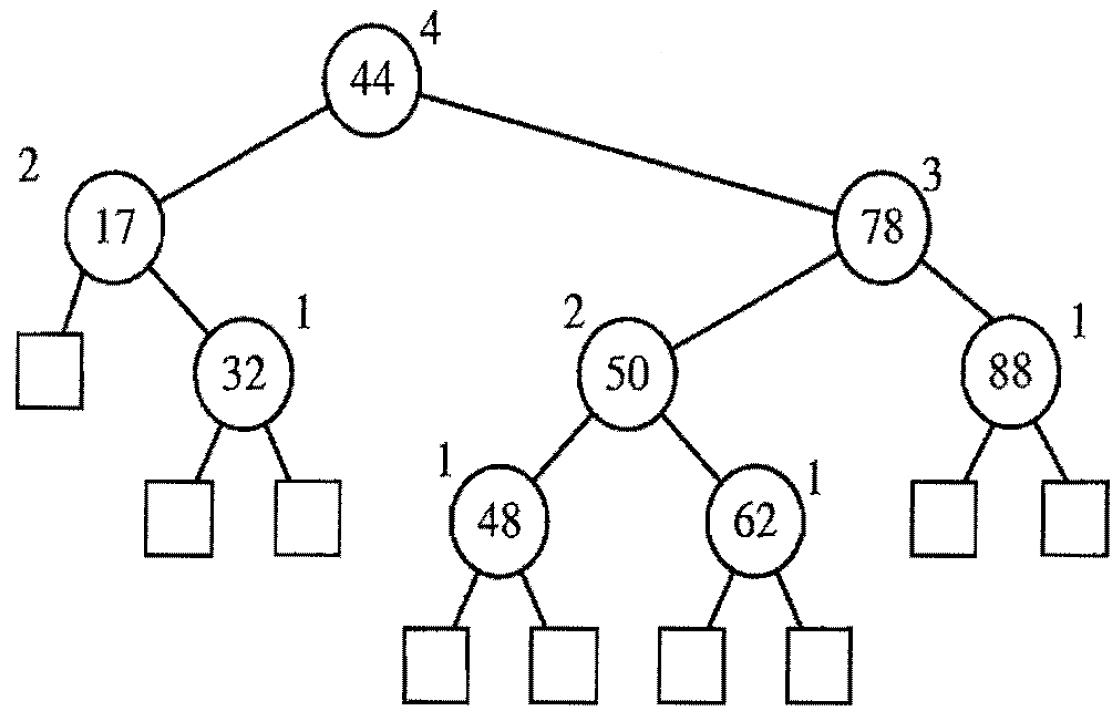
\includegraphics[scale=0.37]{AVL.png}
\caption{Exemple d'arbre AVL. Les clés des entrées sont mises à l'intérieur des noeuds et les hauteurs des noeuds sont indiquées à côté de ces derniers.}
\end{figure}
\newpage
\subsection*{Question 3}
%%Énoncé
Proposez un algorithme pour réaliser la méthode \textit{firstEntry()} (voir DSAJ-5
page 403 et DSAJ-6 page 396) dans un arbre binaire de recherche. Proposez un
algorithme pour réaliser la méthode \textit{higherEntry(k)} (voir DSAJ-5 page 403
et DSAJ-6 page 396) où \textit{k} est une clé présente dans un arbre binaire de recherche.

Quelles sont les complexités temporelles de vos algorithmes en fonction de \textit{h} (la
hauteur de l’arbre) et en fonction de \textit{n} (le nombre de noeuds de l’arbre) ?
(Tanguy)\footnote{Sources : \url{http://docs.oracle.com/javase/7/docs/api/java/util/TreeMap.html} et "TreeMap.java" issu du SDK 7}
\\
\\
%%Réponse
Algorithme pour \textit{firstEntry()}
\lstinputlisting[language=java, inputencoding=utf8]{firstEntryMethod.java}
Algorithme pour \textit{higherEntry(k)}
\lstinputlisting[language=java, inputencoding=utf8]{higherEntryMethod.java}

Pour les deux méthodes, la complexité temporelle est en $O (h)$ par rapport à la hauteur car il faut descendre tout en bas de l'arbre et en $O (\log (n))$ en fonction du nombre de noeuds car on ne tient compte que du sous-arbre de gauche à chaque itération.
\newpage
\subsection*{Question 4}
Partant d’un arbre binaire de recherche initialement vide, comment se présente
l’arbre après y avoir inséré les clés 12, 5, 10, 3, 13, 14, 15, 17, 18, 15 ? Pour
les mêmes données comment se présenterait l’arbre finalement obtenu s’il s’agissait
d’un arbre (2,4) ? Pour les mêmes données comment se présenterait l’arbre
finalement obtenu s’il s’agissait d’un B-arbre d’ordre 4 ou d’un Splay Tree ? Cet
exemple illustre-t-il les avantages ou inconvénients de ces différentes structures
de données ? Pourquoi ? (Alexandre)

%%Réponse
\subsection*{Arbre binaire de recherche}
\begin{tikzpicture}
\node[circle,draw](z){$30$}
	child{
		node[circle,draw]{5} child{node[circle,draw] {3}} child{node[circle,draw] {10}}}
	child{
		node[circle,draw]{13} child[missing] 
			child{
				node[circle,draw]{14}  child[missing] child {
					node[circle,draw]{15}  child[missing] child{
						node[circle,draw]{17}   child{node[circle,draw] {15}}  child{node[circle,draw] {18}}
					}
				}
			}};
\end{tikzpicture}

\subsection*{Arbre (2,4)}
\begin{tikzpicture}
\tikzstyle{bplus}=[rectangle split, rectangle split horizontal,rectangle split ignore empty parts,draw]
\tikzstyle{every node}=[bplus]
\tikzstyle{level 1}=[sibling distance=20mm]
\node {10\nodepart{two} 13 \nodepart{three} 15}
  child {node {3 \nodepart{two} 5}}
  child {node {12}}
  child {node {14}} 
  child {node {16 \nodepart{two} 17 \nodepart{three} 18}};
  \end{tikzpicture}
  
  \subsection*{B-arbre d'ordre 4}
  \begin{tikzpicture}
\tikzstyle{bplus}=[rectangle split, rectangle split horizontal,rectangle split ignore empty parts,draw]
\tikzstyle{every node}=[bplus]
\tikzstyle{level 1}=[sibling distance=60mm]
\tikzstyle{level 2}=[sibling distance=15mm]
\node {12}
  child {node {5}
    child {node {3}}
    child {node {10}}
  } 
  child {node {14 \nodepart{two} 15}
    child {node {13}}
    child {node {15}}
    child {node {17 \nodepart{two}18}}    
  }
;\end{tikzpicture}
  \subsection*{Splay tree}
  \begin{tikzpicture}
  \tikzstyle{bplus}=[circle,draw]
  \tikzstyle{every node}=[bplus]
\node{$15$}
	child{node{15} child{node{14} child{node{13} child{node{5} child{node{3}} child{node{12} child{node{10}} child[missing]}} child[missing]} child[missing]} child[missing]}
	child{node{18} child{node{17}} child[missing]}
;\end{tikzpicture}

\subsection*{Conclusion}

Ces différents schémas permettent de mettre en évidence les différences qu'ils existent entre eux comme la profondeur de l'arbre, le nombre maximum d'élément fils d'un nœud...
  
\newpage
\subsection*{Question 5}
%%Énoncé
Énoncé

%%Réponse
Réponse
\newpage
\subsection*{Question 6}
%%Énoncé
Énoncé

%%Réponse
Réponse
\newpage
\subsection*{Question 7}
%%Énoncé
Énoncé

%%Réponse
Réponse
\newpage
\subsection*{Question 8}
%%Énoncé

Supposons que nous disposions d'un arbre binaire de recherche mémorisant des clés entières entre 1 et 1000 et que nous y cherchions la clé 363. Parmi les séquences suivantes, quelles sont celles qui ne peuvent pas correspondre à la séquence des clés examinées ?

\begin{itemize}

\item 2, 252, 401, 398, 330, 344, 397, 363
\item 924, 220, 911, 244, 898, 258, 362, 363
\item 925, 202, 911, 240, 912, 245, 363
\item 2, 399, 387, 219, 266, 382, 381, 278, 363
\item 935, 278, 347, 621, 29

\end{itemize}
\textit{(Jonathan)} \\
%%Réponse
\\ Toutes ces séquences sont possible sauf deux d'entre elle.
La troisième séquences ainsi que la dernière des séquences.

En effet pour la séquence : 925, 202, 911, 240, \underline{912}, 245, 363
Le résultat 912 ne peut pas se trouver dans la séquence des clés. En effet après 911 nous nous trouvons dans son sous arbre gauche. Il est donc impossible de trouver la clés 912 dans ce sous arbre de gauche.


Pour la séquence 935, 278, 347, 621, \underline{299}, 392, 358, 363
Lors de la recherche après avoir passé la clés 347 nous nous trouvons dans son sous arbre de gauche. Étant donné que la clés suivante est 612 nous nous trouvons forcément à une valeur supérieure à 347, mais inférieure à 621. Il est donc impossible de rencontrer la valeur 299.
%\newpage
%\subsection*{Question 9}
%%%Énoncé
Énoncé

%%Réponse
Réponse
%\newpage
%\subsection*{Question 10}
%%%Énoncé
Énoncé

%%Réponse
Réponse
%\newpage
%\subsection*{Question 11}
%%%Énoncé
Énoncé

%%Réponse
Réponse
%\newpage
\end{document}
